%!TEX root = ../dissertation.tex

\chapter{Experiment and results}
\label{ch:experiments}

In this chapter we discuss our experimental assessment, carried out on
two widely adopted dataset which are discussed in
Sec.~\ref{sec:datasets}, along with our preprocessing pipeline in
Sec.~\ref{sec:data-preprocessing} and some analysis in
Sec.~\ref{sec:data-analysis}. In Sec.~\ref{sec:impl-details} we talk
about model's implementation details, while in
Secs.~\ref{sec:model-selection} and \ref{sec:evaluation-metric} we
show selected parameters and discuss the chosen evaluation metric.

\section{Datasets}
\label{sec:datasets}

This section describes Flickr30k Entities and ReferIt, the two
datasets on which we developed our model. For both we discuss how they
were collected, what are their purposes, some statistics and we
highlight the data representation.

\subsection{Flickr30k Entities}
\label{subsec:flickr30k}

Flickr30k Entities \cite{plummer2015flickr30k} is a dataset built on
top of Flickr30k \cite{young2014image}, where the main focus is on the
task of grounding textual mentions of entities in image with augmented
data.

Flickr30k Entities consists in highly structured annotations collected
through crowdsourcing with different number of objects per image, and
thus, different complexity per example. Annotations are made of
mentions of the same entities between different captions, and bounding
boxes that localized those entities in the image. Flickr30k Entities
is developed under a strict pipeline of simple and atomic tasks to
tackle the ambiguity in identifying whether two mentions refer to the
same entity or how many boxes (if any) each entity requires. Moreover,
such task are carried out by humans, so there is also the problem of
unreliability of crowdsourced judgments problems. For this reason, the
pipeline is structure into two main stages: coreference resolution and
bounding box annotation. The goals of the pipeline are to reduce
redundancy in annotations and save box-drawing effort while keeping
the process valuable. In Fig.~\ref{fig:flickr30k-example}
\cite{plummer2015flickr30k}, are shown the interfaces used to gather
annotations with respect to tasks described next.

\begin{figure}
  \centering
  \begin{subfigure}{.45\textwidth}
    \centering
    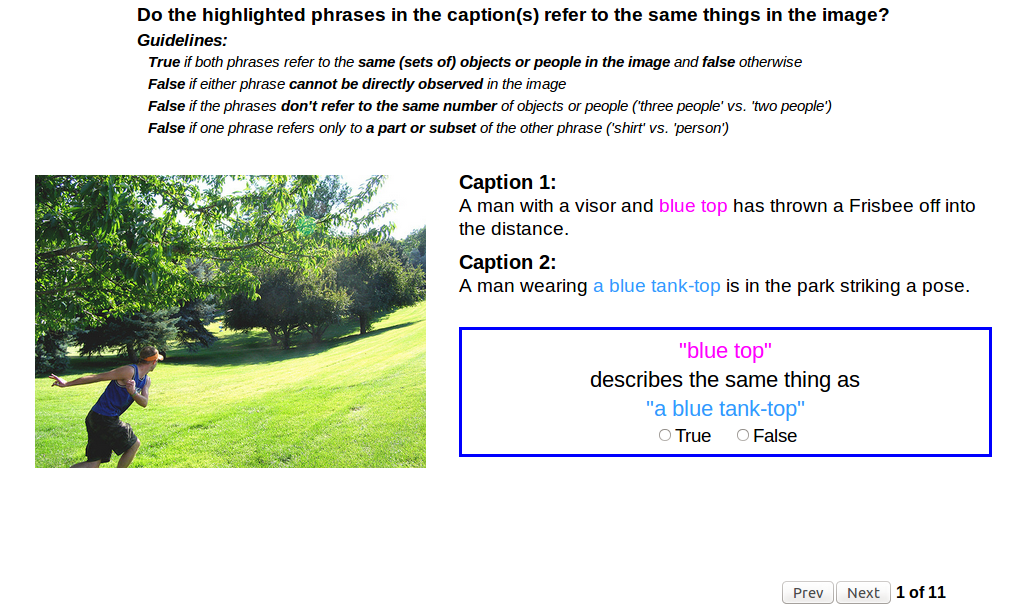
\includegraphics[width=.8\linewidth]{figures/flickr30k-example-coref-annotation.png}
    \caption{Binary coreference link interface}
    \label{fig:flickr30k-example-coref-annotation}
  \end{subfigure}
  \begin{subfigure}{.45\textwidth}
    \centering
    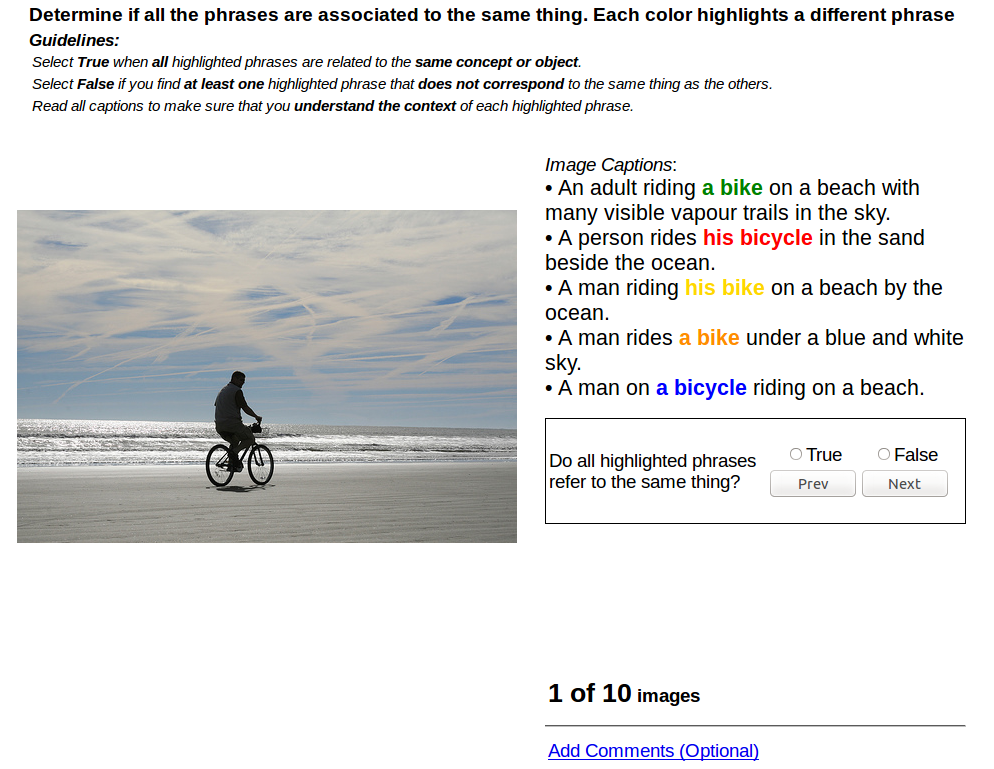
\includegraphics[width=.8\linewidth]{figures/flickr30k-example-coref-verification.png}
    \caption{Coreference chain verification interface}
    \label{fig:flickr30k-example-coref-verification}
  \end{subfigure}
  \begin{subfigure}{.45\textwidth}
    \centering
    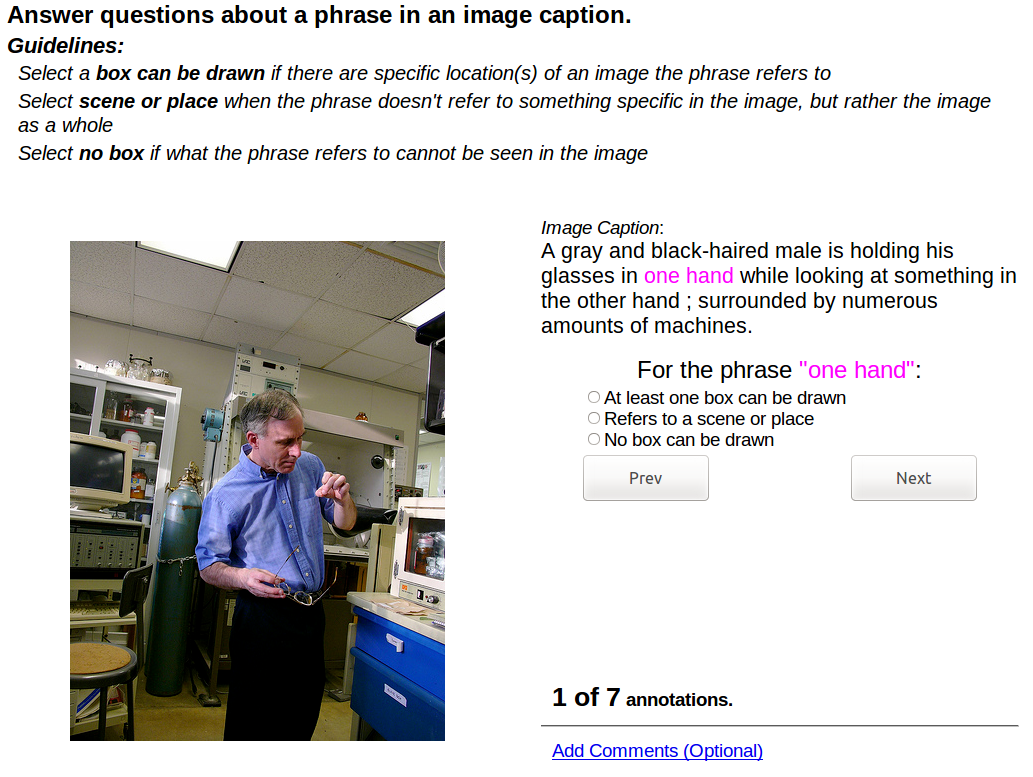
\includegraphics[width=.8\linewidth]{figures/flickr30k-example-box-requirement.png}
    \caption{Box requirement interface}
    \label{fig:flickr30k-example-box-requirement}
  \end{subfigure}
  \begin{subfigure}{.45\textwidth}
    \centering
    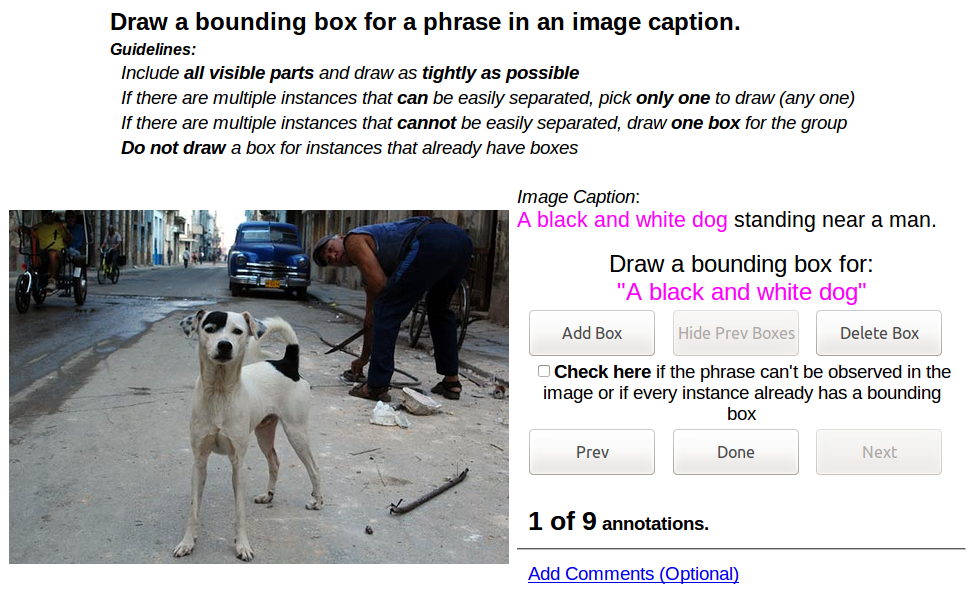
\includegraphics[width=.8\linewidth]{figures/flickr30k-example-box-drawing.png}
    \caption{Box drawing interface}
    \label{fig:flickr30k-example-box-drawing}
  \end{subfigure}
  \begin{subfigure}{.45\textwidth}
    \centering
    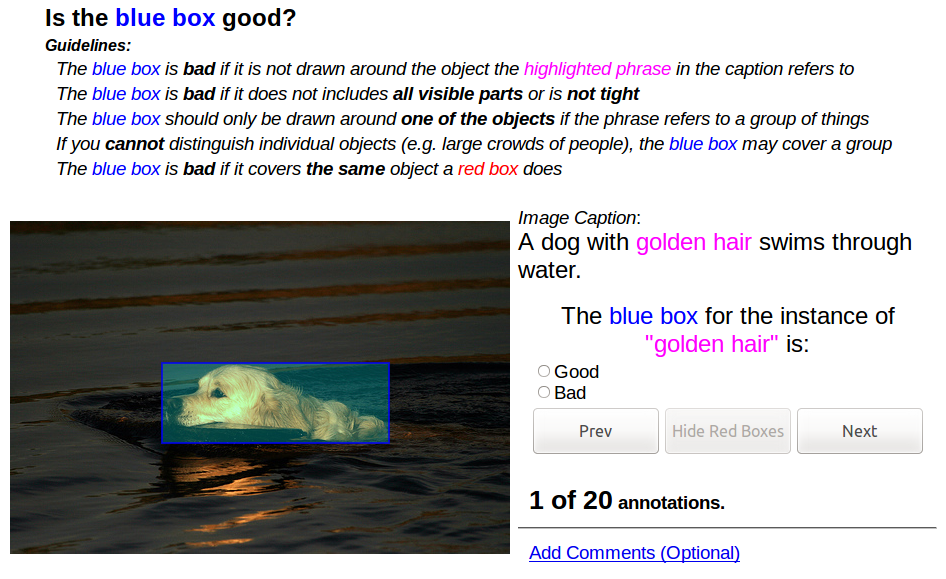
\includegraphics[width=.8\linewidth]{figures/flickr30k-example-box-quality.png}
    \caption{Box quality interface}
    \label{fig:flickr30k-example-box-quality}
  \end{subfigure}
  \begin{subfigure}{.45\textwidth}
    \centering
    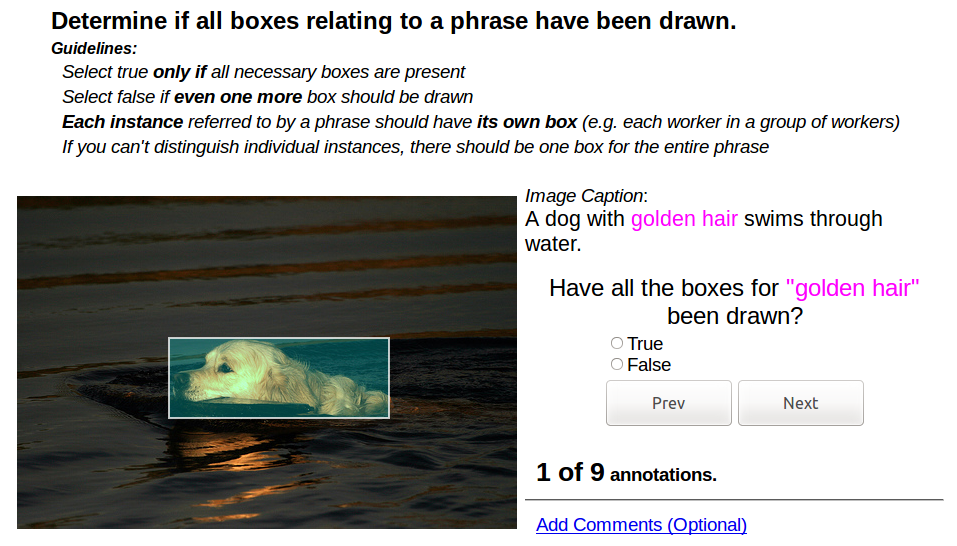
\includegraphics[width=.8\linewidth]{figures/flickr30k-example-box-coverage.png}
    \caption{Box coverage interface}
    \label{fig:flickr30k-example-box-coverage}
  \end{subfigure}
  \caption[Flickr30k Entities annotation system interfaces]{Flickr30k Entities annotation system interfaces \cite{plummer2015flickr30k}.}
  \label{fig:flickr30k-example}
\end{figure}

The coreference resolution task is solved by first chunking
information given in Flickr30k captions to identify potential entity
mentions. Each chunk, i.e., noun phrase, is a potential entity
mention. For example, the phrase ``A man in an orange hat'' is chunked
in two noun phrases, namely ``A man'' and ``an orange hat'', which are
the two mentions. Given $M$ a document containing noun phrases
originated from captions of an image, a worker is required to specify
whether two given mentions $m$ and $m'$ refer to the same entity. If
the answer is positive, a link between the two mentions is added,
creating a coreference chain. Typically, this would require $O(|M|^2)$
which is the cost of all pairwise links. But since $M$ usually
contains multiple mentions that refer to the same set of entities, the
number of coreference chains is bounded by a number much smaller than
$|M|$, on average. Moreover, the bound is lowered by making two extra
assumption: first, mentions from the same captions cannot or belonging
to different categories be coreferent. Categories assigned to each
mention are coarse-grained types, such as: people, body parts,
animals, clothing/color, instruments, vehicles, scene, and other.

Bounding box annotation is carried out with a workflow composed by
four tasks administered to workers, namely: box requirement, box
drawing, box quality and box coverage. In box requirement, a worker
needs to specify, whether at least one bounding box can be drawn in
image for given mention. If the response is negative, the mention
leaves the workflow, otherwise it goes through the box drawing stage.
Here, a worker should draw a box as tight as possible around the
mentioned entity. The main source of difficulty in this stage is due
to mentions that refer to multiple entities. If a box is drawn, then
the mention-box pair proceeds to box quality stage. At this point,
drawn box is evaluated in terms of redundancy (are there any box that
already covers the same entity?), accuracy (is the box tight around
the entity?), distinctiveness (can a box be drawn for single entity
instead of covering multiple elements?). If the answer is positive,
the example goes to the last stage. In box coverage, workers decide
whether all required boxes are present in image. 

During the annotation process, workers are subjected to quality
control process. Workers must pass a test before being allowed to
annotate dataset examples. Also, during the annotation process,
workers are asked some verification questions (question with known
answer, written by authors).

In the end, Flickr30k Entities is made up of 32K images, 159K
sentences, 275K bounding boxes, and 360K noun phrases where each image
is associated with five sentences with a variable number of noun
phrases, and each noun phrase is associated with a set of bounding
boxes ground truth coordinates. 

\subsubsection{Data Representation}
\label{subsec:flickr30k-data-representation}

Technically speaking, in Flickr30k Entities each example is composed
by information contained in three different files linked together by
means of an identifier $id$. Those files represent image, sentence
annotations and image annotations information. The image file is
simply a JPG file, while the sentence annotations file is a textual
document containing five captions. Each caption is chunked into a
variable number of noun phrases and each noun phrase can be linked to
a bounding box contained in the third file. The image annotation file
is an XML file with an array of objects. Every object has one or more
name, that can be used to reconstruct which noun phrase is linked to
the bounding box, and four coordinates $x_{min}, y_{min}, x_{max},
y_{max}$ if it is a visual element, none otherwise. The structure is
visually explained in
Fig.~\ref{fig:flickr30k-technical-data-representation}.

\begin{figure}
  \centering
  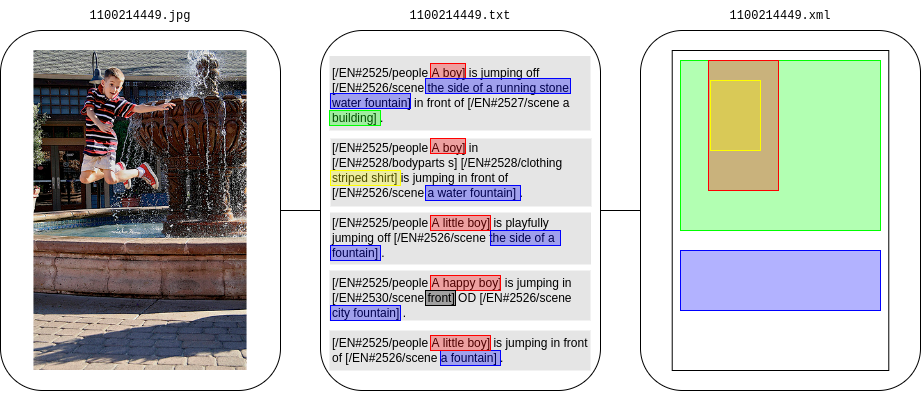
\includegraphics[width=0.8\textwidth]{figures/flickr30k-document-specification.png}
  \caption[Flickr30k Entities document specification]{ Flickr30k
    Entities document specification. Each image is identified by a
    number that is identical for textual and visual annotations. The
    txt file describe five captions, each one containing one or more
    noun phrases. The xml file describes the ground truth bounding box
    annotations. }
  \label{fig:flickr30k-technical-data-representation}
\end{figure}

Those data ara available online in two parts: images and can be
downloaded by compiling a registration form,
\footnote{\href{http://shannon.cs.illinois.edu/DenotationGraph/}{http://shannon.cs.illinois.edu/DenotationGraph/}}
while annotations, instead, do not requires a sign up: data can be
downloaded from B. A. Plummer repository on GitHub.
\footnote{\href{https://github.com/BryanPlummer/flickr30k\_entities}{https://github.com/BryanPlummer/flickr30k\_entities}}
Within the repository, authors have made available predefined
training, validation and test split that we use in our work, following
current literature.

\subsection{ReferIt}
\label{subsec:referit}

ReferIt \cite{kazemzadeh2014referitgame} is another popular dataset.
The reason that led to developing this dataset is to study how people
refer to objects in complex photographs of a real-world cluttered
scenes. Thus, the focus is on referring expression grounding task.
However, due to the heterogeneity of data, it can be employed also in
phrase grounding.

ReferIt contains very challenging examples from phrase grounding point
of view, because the dataset is collected entirely in an unsupervised
context by crowd through a game. Examples vary from ``a man'' and
``the person in red'' to ``buildings'' or more degenerative ones like
``i don't think that was trash, lol. anyway, wall just above heads''.
In ReferIt many phrases uses spatial relations among objects, such as
``building on right behind guys'' or ``window top 2nd left''.

Referring expressions are collected through \textit{ReferItGame},
which is a two-player online game. The game is the key point of the
whole dataset, because it allow to collect large-scale dataset
containing natural language expressions referring to objects in
photographs of real world scenes in an inexpensive way.

The game is a simple two player game where players alternate between
generating expressions referring to objects in images of natural
scenes, and clicking on the locations of described objects.
Fig.~\ref{fig:referitgame-example}, from
\cite{kazemzadeh2014referitgame} shows an example of the game. The
game play is straightforward: Player 1 is given an image with an
object outlined in red and and he has to write a caption. Player 2
receives the same image without outlined object and the referring
expression written by Player 1, his goal is to localize the described
object. Both players receive game points whether Player 2 correctly
localize the object instead no points are earned. When there are no
players available for a player vs player match, then a canned match is
started where the missing player is replaced by a CPU player.

\begin{figure}
  \centering
  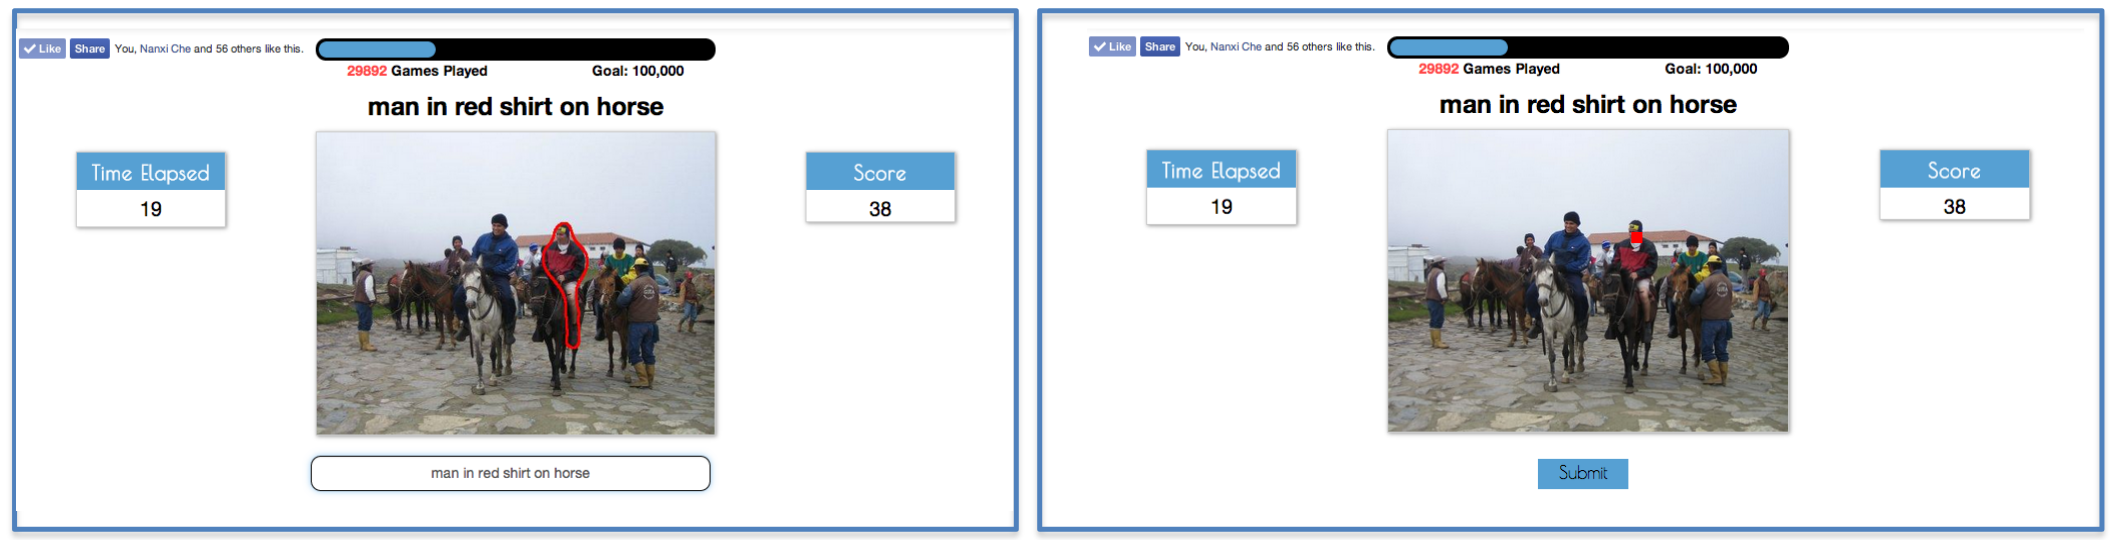
\includegraphics[width=0.8\textwidth]{figures/referitgame-example.png}
  \caption[ReferIt Game GUI interface]{ ReferIt Game GUI interface
  from \cite{kazemzadeh2014referitgame}. Player 1 \textit{(left)} sees
  an image with an object outlined in red (the man) and provides a
  referring expression for the object (``man in red shirt on horse'').
  Player 2 \textit{(right)} sees the image and the expression from
  Player 1 and must localize the correct object by clicking on it
  (click indicated by the red square). Elapsed time and current scores
  are also provided. }
  \label{fig:referitgame-example}
\end{figure}

\subsubsection{Data Representation}
\label{subsec:referit-data-representation}

ReferIt resources and references are made available online at its
website
\footnote{\href{http://tamaraberg.com/referitgame/}{http://tamaraberg.com/referitgame/}},
while instructions and data are provided at Licheng Yu's GitHub
repository.\footnote{\href{https://github.com/lichengunc/refer}{https://github.com/lichengunc/refer}}
Images are stored in JPG files, while annotations are described
through two structured file. One is a JSON file containing the
bounding box annotations along with a list of images and their $id$,
the other is a PICKLE
file\footnote{\href{https://docs.python.org/3/library/pickle.html}{https://docs.python.org/3/library/pickle.html}}
containing a serialized Python object that represents sentence
annotations. The Fig.~\ref{fig:referit-technical-data-representation}
depict described structure.

\begin{figure}
  \centering
  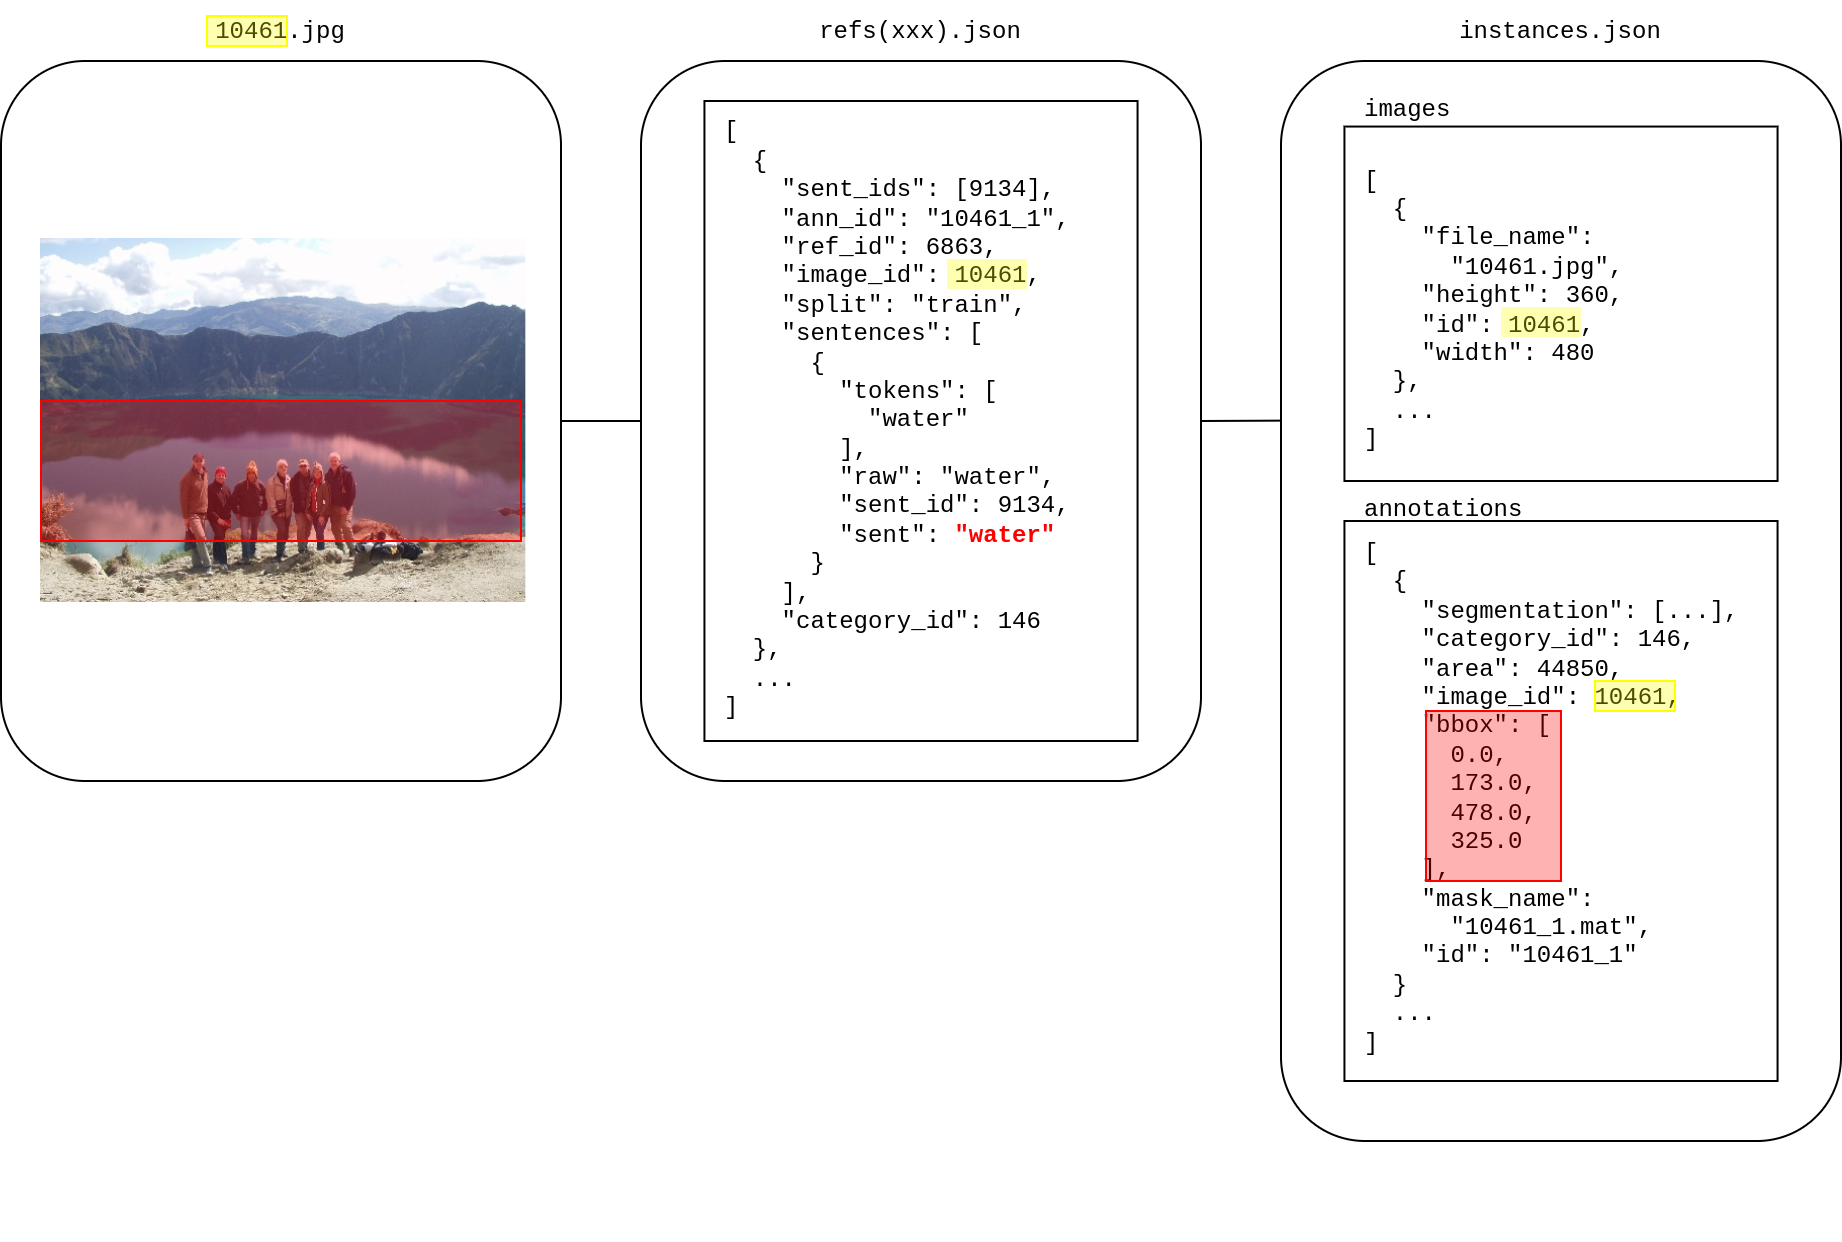
\includegraphics[width=0.8\textwidth]{figures/referit-document-specification.png}
  \caption[ReferIt document specification]{ReferIt document
  specification. Each image is identified by a number. This identifier
  is used to link visual and textual annotations in the two json file.
  Particularly, ``ref(xxx).json'' contains a list of sentences along
  with their annotations, while in ``instances.json'' there are two
  list. The first is an index of all images (with some properties),
  while the second contains annotation for ground truth bounding
  boxes. }
  \label{fig:referit-technical-data-representation}
\end{figure}

\section{Data Preprocessing}
\label{sec:data-preprocessing}

It is well known that data preparation and filtering steps requires a
considerable amount of effort both for engineer the process and to
develop an effective and efficient preprocessing pipeline
\cite{kotsiantis2006data}. Most of the time, data we collect or borrow
are biased, flowed, redundant, maybe irrelevant and sometimes
corrupted or missing. For the development of an accurate and general
model, the representation and quality of the instance data must be
maximized. This involves working on tasks like cleaning,
normalization, transformation, feature extraction and selection.
Fortunately, we do not work with row data: due to the large adoption
of datasets described in Sec.~\ref{sec:datasets}, provided data are
already preprocessed in a grossly way.

In the next section we describe our preprocessing pipeline, focusing
on data representation which can be quite confusing due to the
heterogeneity of representations. In particular,
Sec.~\ref{subsec:data-preparation} describes transformation and
augmentations applied to data, while Sec.~\ref{subsec:data-interface}
describes the interface we used to represent heterogeneous data.

\subsection{Data Preparation}
\label{subsec:data-preparation}

Given data as specified in
Sec.~\ref{subsec:flickr30k-data-representation} and
\ref{subsec:referit-data-representation} for, respectively, Flickr30k
Entities and ReferIt, we create a single and unified data interface
which exposes features homogeneously and enables the model to work
with different datasets transparently. Then, we augment data with
further information coming from a pretrained object detector.

In the first place, we run an object detector
(Sec.~\ref{sec:object-detection-recognition}) to extract features. The
proposal extractor generates a list of bounding box and the object
detector computes $2048$ features per bounding along with two
probability distributions, respectively for classes and attributes.
For each bounding box $\bm{b}_i$, the object returns a probability
distribution over a set of classes $Cls$, i.e., $Pr_{Cls}(\bm{b}_i)$
and a probability distribution over a set of attributes $Attr$, i.e.,
$Pr_{Attr}(\bm{b}_i)$. In contrast to classes, each bounding box can
be represented by more than one attribute: attributes can be
considered present if their probability is above a predefined
threshold.

Then, we process ground truth bounding boxes annotated in the dataset
in order to match them with object detector proposals. For each ground
truth bounding box $\bm{b}^{gt}_i$, we have to find the proposal
generated by object detector $\bm{p}_{i^*}$ such that the intersection
over union (Sec.~\ref{subsec:iou}) between the two is maximized:
$\bm{p}_{i^*} = \argmax_{\bm{p} \in \calP_{\bm{I}}}
\iou(\bm{b}^{gt}_i, \bm{p})$. Moreover, following all works in
literature, if a noun phrase corresponds to multiple ground truth
bounding boxes, we merge the boxes and use their union region as its
ground truth. On the contrary, if a noun phrase has no associated
bounding box, we remove it from the dataset.

\subsection{Data Interface}
\label{subsec:data-interface}

The data interface is designed to be as flexible and complete as
possible, allowing the adaptation of other datasets with low effort.
In particular our interface includes the following.

\begin{itemize}
  \item An positive integer used as identifier for the example.
  \item A sentence, i.e, the caption of the image.
  \item A list of phrases, i.e., noun phrases in sentence.
  \item A list of coordinates, representing, for each phrase, the
  ground truth bounding box.
  \item The width and the height of the image.
  \item A list of bounding box coordinates.
  \item A list of features per bounding box.
  \item A list of probabilities, i.e., a probability distribution
  $Pr_{Cls}(\bm{i})$ for each proposal $\bm{p}_i$ over a set of
  classes $Cls$.
  \item A list of attribute probabilities, i.e., a probability
  distribution $Pr_{Attr}(\bm{i})$ for each proposal $\bm{p}_i$ over a
  set of attributes $Cls$.
  \item A list of features per bounding box.
\end{itemize}

The Fig.~\ref{lst:data-interface-dict} shows a real word example
exposing data through the unified interface. (For the sake of
presentation we omitted full data in favor of ellipsis).

\begin{lstlisting}[style=simplepython,caption=Example of our data structure for as interface to row data.,label={lst:data-interface-dict},captionpos=b]
{
    id: '3359636318', 
    sentence: 'Two people are talking outside of the video game shop next door to the mobile phone store .', 
    phrases: ['Two people', 'the video game shop', 'the mobile phone store'], 
    n_phrases: 3, 
    phrases_2_crd: [[46, 165, 207, 333], [0, 54, 168, 307], [191, 0, 498, 230]], 
    image_w: 500, 
    image_h: 334, 
    image_d: 3, 
    pred_n_boxes: 100, 
    pred_boxes: [[0.0, 280.0, 278.4, 333.4], [395.5, 232.3, 453.2, 333.1], ...], 
    pred_cls_prob: [[0.09, 0.01, ...], [0.27, 0.02, ...], ...],
    pred_boxes_features: [[0.0, 2.0, ...], [2.57, 1.17, ...], ...]
}
\end{lstlisting}

\section{Implementation Details}
\label{sec:impl-details}

We started from the codebase provided by D. Rigoni \etal{}
\cite{rigoni2021better} where they implement a phrase localization
system with the ability to include information from knowledge graph,
thus solving the VTKEL task (Sec.~\ref{sec:vtkel}). For this reason,
some implementation details are inherited from their work. For
example, we use the same pre-trained object detector Faster R-CNN
(Sec.~\ref{subsec:faster-rcnn}) pre-trained on Visual Genome
\cite{krishna2017visual} dataset, with ResNet-101 as backbone model
pre-trained on COCO for initialization. Bounding box features matches
the ResNet-101 layer \textit{pool5\textunderscore flat} for a total of
$v = 2048$ features. Moreover, for each proposal we extract a
probability distribution over $1600$ classes $Cls$. Please note that
the implementation in \cite{anderson2018bottom} returns $1600 + 1$
classes. The extra label is the ``background'' class, used as a
default for proposals whose label cannot be predicted with good
confidence. In our work, we ignore proposals labeled with as
background because under weak supervision we cannot rely such a noisy
information. As an example, with $100$ proposals per image, we removed
$47.6\%$ proposals on average on Flickr30k Entities while $51.1\%$ on
ReferIt.\footnote{Along with classes information, the object detector
makes available also attributes information on proposals. On the same
way of classes, they return a probability distribution on $400 + 1$
attributes. Unfortunately, the implementation of attributes prediction
for the object detector in \cite{anderson2018bottom} is erroneous. As
they state in Sec. 6.1, the probability for each attribute should be a
number between $0$ and $1$ and an attribute is considered when its
probability is over $0.2$. Instead, the current implementation returns
a softmax over the labels, i.e., $400 + 1$ attributes label. The extra
label is the ``background'' attribute. Probably this error is due to
careless copy-pase from class prediction branch. For this reason, we
do not include this information in our model.} We use SpaCy
\cite{honnibal2020spacy} parser in order to extract words vocabulary
from both datasets and also to retrieve heads from phrase. In contrast
to \cite{rigoni2021better}, we initialize word embeddings with
pre-trained Word2Vec \cite{mikolov2013efficient} weights instead of
GloVe \cite{pennington2014glove}, but we keep the same settings:
embeddings are freezed (we do not train them) and out-of-vocabulary
words are initialized according to Xavier
\cite{glorot2010understanding}. The size of the embedding is $w =
300$. In the prediction module we instanced $\lambda = 0.5$, equally
weighting both model predictions and prior scores.

During our work, we trained the model on the training set for $30$
epochs, while we performed model selection onto the validation set.
The comparison with other works is done on the test set. We found the
best epoch on Flickr30k Entities to be the $15$-th, while on ReferIt
the $27$-th. 

\section{Data Analysis}
\label{sec:data-analysis}

Data analysis is another crucial task of data processing pipeline and
it is not only important to process and manipulate data, but also to
analyze the relationships and correlations and to identify patterns
and trends for results interpretation \cite{sharma2020understanding}.
Data analysis can be decisive also in the phase of model design,
because it can outline problems or intrinsic traits that belongs to
data and must be taken into account.

Within the following sections we outline our shallow data analysis,
performed on-demand while designing the model in overcome problems.

\subsection{Number of Bounding Box per Image and Upperbound Accuracy}
\label{subsec:num-of-proposals}

Each image in the dataset is different and vary wrt number of objects
in it, type of scene, dimensions and so on. Thus, by nature of images,
the object detector can extract a variable number of bounding boxes
and usually, only a variable subset of these are relevant. However,
for implementation reason we are required to fix a number $k$ of
proposal per example. So, how to choose $k$? If $k$ is too low we
cannot reach good coverage wrt ground truth bounding boxes, while if
$k$ is too big we have to deal with many similar boxes and we require
more resources to run the model. It's a tradeoff problem. Please note
that, independently from $k$, proposals are always selected by maximum
importance score \cite{ren2015faster}.

Following literature we initially fixed the upper-threshold to $k =
100$ proposals, and then we performed an analysis on both dataset
aimed to detect the distribution of proposals per image. We discovered
that for almost every example the object detector can detect maximum
number of proposal, except to some degenerative images. For example,
the object detector extracted less than $100$ proposals for $194$
images over $31783$ in Flickr30k Entities and $120$ over $19995$ in
ReferIt.

What remains to prove is whether we can reach a good upperbound
accuracy given $100$ proposals wrt the ground truth bounding box. We
analyzed the data and we discovered that with $k = 100$ bounding box
the coverage is good enough (nearly $93\%$ on Flickr30k Entities and
$91\%$ on ReferIt), while decreasing $k$ resulted in an upperbound
accuracy drop (nearly $54\%$ Flickr30k Entities and $51\%$ ReferIt).
The Tab.~\ref{tab:bb-coverage} summarizes the outcome.

\begin{table}
  \centering
  \begin{tabular}{c|cc}
     & \multicolumn{2}{c}{Upperbound Accuracy (\%)} \\
    $k$ & Flickr30k Entities & ReferIt \\\hline 
    $100$ & $93.4$ & $91.4$ \\ 
     $90$ & $93.1$ & $90.9$ \\  
     $80$ & $92.7$ & $90.3$ \\
     $70$ & $92.0$ & $89.5$ \\
     $60$ & $91.2$ & $88.5$ \\
     $50$ & $89.8$ & $86.8$ \\
     $40$ & $87.5$ & $84.2$ \\
     $30$ & $83.3$ & $79.7$ \\
     $20$ & $74.5$ & $70.5$ \\
     $10$ & $53.9$ & $51.0$ \\\hline
  \end{tabular}
  \caption[Upperbound accuracy per number of proposals on Flickr30k
    Entities and ReferIt]{ Upperbound accuracy per number of proposals
    on Flickr30k Entities and ReferIt.}
  \label{tab:bb-coverage}
\end{table}

\subsection{Upperbound Accuracy Removing Background Class}

The implementation of object detector we are using
\cite{anderson2018bottom} returns a distribution of probability over a
set of $1600 + 1$ labels per proposal, identifying the semantic
content of the box through a word. The extra label is the background
class and it is used to represent the absence of classification.

Proposals tagged with background class are very common. For example,
by setting $k = 100$, we got $47.6$ and $51.1\%$ background tagged
proposals on Flickr30k Entities and ReferIt, respectively.
Intuitively, one may think that proposals labeled as non-informative
should be discarded, but \cite{yu2018rethinking} proved that visual
features from object detector internal layers convoy important
information about the portion of the image and may relax the
upperbound accuracy constraint. We argue that in our weakly supervised
approach the background label may introduce noise, so as a
preprocessing step we keep only properly-labeled proposals.

Since, we decided to remove such boxes, we investigated the problem of
box coverage, and hence, maximum achievable accuracy. We analyzed this
phenomenon and we surprisingly noticed that even removing nearly one
proposal over two, the upperbound accuracy remains comparable to the
version without background removal. In particular, we obtained an
absolute loss of $3.7$ and $5.8\%$ accuracy on average, respectively
for Flickr30k Entities and ReferIt, wrt to upperbound accuracy without
background removal. Analytics details are reported in
Tab.~\ref{tab:bb-coverage-no-background}.

\begin{table}
    \centering
    \begin{tabular}{c|cc|cc}
       & \multicolumn{2}{c|}{Flickr30k} & \multicolumn{2}{c}{ReferIt} \\\hline
      $k$ & \multicolumn{1}{p{2.2cm}|}{\centering Upperbound\\ Accuracy (\%)} & \multicolumn{1}{p{2.2cm}|}{\centering Average Box\\ Removed (\%)} & \multicolumn{1}{p{2.2cm}|}{\centering Upperbound\\ Accuracy (\%)} & \multicolumn{1}{p{2.2cm}}{\centering Average Box\\ Removed (\%)}   \\\hline 
      $100$ & $88.3$ & $47.6$ & $83.0$ & $51.1$ \\
       $90$ & $87.9$ & $46.6$ & $82.6$ & $49.9$ \\
       $80$ & $87.5$ & $44.8$ & $82.2$ & $48.4$ \\
       $70$ & $86.9$ & $42.7$ & $81.6$ & $46.4$ \\
       $60$ & $86.3$ & $40.0$ & $80.9$ & $43.7$ \\
       $50$ & $85.3$ & $36.3$ & $80.1$ & $39.9$ \\
       $40$ & $83.8$ & $30.8$ & $78.8$ & $34.5$ \\
       $30$ & $80.8$ & $22.4$ & $76.0$ & $26.4$ \\
       $20$ & $73.6$ & $10.8$ & $68.9$ & $15.0$ \\
       $10$ & $53.9$ &  $1.2$ & $50.8$ &  $3.8$ \\\hline
    \end{tabular}
  \caption[Achievable upperbound accuracy by removing background labeled proposals on Flickr30k Entities and ReferIt]{Achievable upperbound accuracy by removing background labeled proposals on Flickr30k Entities and ReferIt.}
  \label{tab:bb-coverage-no-background}
\end{table}

\subsection{Distribution of Class Labels on Proposals}

For a good comprehension of object detector information, we studied
the distribution of number of examples per label. We performed the
analysis on both dataset but for presentation purposes, here we show
qualitative data from Flickr30k Entities; ReferIt shows comparable
insights. The distribution, shown in
Fig.~\ref{fig:flickr30k-label-distribution-top10}, is a long-tail
distribution. This means that there are few labels with a very large
population, while many other labels count little number of examples.
We truncate the plot to top-$100$ labels (among $1600$) with larger
population and the phenomenon is clearly visible. In
Tab.~\ref{tab:flickr30k-label-data-top10} we report the top-$10$
labels per number of examples. Except to the evident gender gap whose
implications are out of scope for this work, we show that there is a
great discrepancy in terms of number of examples for labels like man,
woman, people and the others.

\begin{figure}
  \centering
  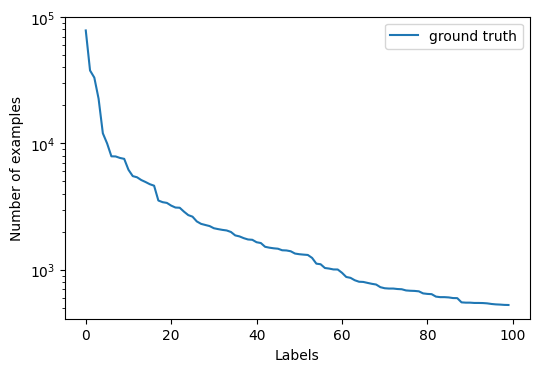
\includegraphics[width=0.8\textwidth]{figures/number-of-examples-per-label-over-top-100-most-popular-labels.png}
  \caption[Number of examples per label over top-100 most popular
    labels on Flickr30k Entities]{ Distribution of examples ($y$ axis, log
    scaled) per label over top-100 most popular labels ($x$ axis) on
    Flickr30k Entities.}
  \label{fig:flickr30k-label-distribution-top10}
\end{figure}

\begin{table}
  \centering
  \begin{tabular}{lc}
    Class  & N       \\\hline
    man    & $78250$ \\
    woman  & $37751$ \\
    people & $33149$ \\
    shirt  & $22585$ \\
    boy    & $12019$ \\
    dog    & $9989$  \\
    wall   & $7905$  \\
    girl   & $7886$  \\
    water  & $7674$  \\
    ground & $7547$  \\
  \end{tabular}
  \caption{Distribution of examples over top-10 labels with larger population.}
  \label{tab:flickr30k-label-data-top10}
\end{table}

\section{Evaluation Metric}
\label{sec:evaluation-metric}

Aligned with the works in literature, we consider the standard
accuracy metric. Given a noun phrase, it considers a bounding box
prediction to be correct if and only if the intersection over union
(Sec.~\ref{subsec:iou}) value between the predicted bounding box and
the ground truth bounding box is at least $\alpha$. Formally, given
the image $\bm{I}$ and sentence $S$, the accuracy between $B^* = \{
\bm{b}^* \}$ the set of predicted bounding boxes for $\bm{I}$ and $S$,
with $|B^*| = m$ where $m$ is the number of noun phrases in $S$ and
$B^{gt}$ the set of ground truth bounding boxes for $\bm{I}$ and $S$
with $|B^{gt}| = m$, can be defined as
\[
  acc(B^*, B^{gt}) = \frac{\sum_{i = 1}^{m} \One (\iou (\bm{b}_i^*, \bm{b}_i^{gt}) \geq \alpha)}{m}.
\]
Following literature we chose $\alpha = 0.5$.

Moreover, we also calculate the pointing game accuracy
(Sec.~\ref{subsec:pointing-game-metric}) for comparison purposes.
Pointing game accuracy consider an example to be positive whether the
center of predicted bounding box lies wherever inside the ground truth
box. More formally, given the image $\bm{I}$ and sentence $S$, we
define pointing game accuracy as 
\[
  acc_{point}(B^*, B^{gt}) = \frac{\sum_{i = 1}^{m} \One (c_i^* \in  \bm{b}_i^{gt})}{m},
\]
where $m$ the number of noun phrases in $S$, $c^*_i = (x +
\frac{w}{2}, y + \frac{h}{2})$ is the center of box $\bm{b}^*_i$ with
$x, y$ its top-left point coordinates and $w, h$ its width and height.
Note that $c^*_i \in \bm{b}^{gt}_i$ is an abuse of notation, we mean true
when $c^*_i$ falls inside $\bm{b}^{gt}_i$ boundaries.

The pointing game accuracy allows to evaluate the goodness of the
model in spatially locating objects, but is a very optimistic metric
wrt the standard accuracy. This is because it requires at least a
point falling inside the ground truth bounding box to consider the
grounding as a hit, while the standard accuracy requires, depending on
$\alpha$, a certain fraction of area to overlap the ground truth
bounding box.

\section{Model Selection}
\label{sec:model-selection}

The model used in test set for both Flickr30k Entities and ReferIt
datasets is chosen on the epoch that better performed in terms of
accuracy in validation set. We carried out hyper-parameters selection
only on Flickr30k Entities, while on ReferIt we applied best
hyper-parameters selected on the former dataset. We used Adam
optimizer with gradient clipping.

In what follows, we summarize hyper-parameters selection. We selected
$10^{-3}$ for the learning rate among $\{ 10^{-1}, 10^{-2}, 10^{-3},
10^{-4}, 10^{-5} \}$. The word embeddings we selected is Word2Vec, but
GloVe scores comparable performance. In both cases, the word embedding
dimension was set to $w = 300$. For the sentence encoder we tried a
plain RNN versus an RNN with LSTM cells. We found good performance in
the latter with $1000$ as dimension for hidden units among $\{ 500,
1000, 1500 \}$  and $1$ layer among $\{ 1, 2 \}$. For the image
features we extracted $k = 100$ proposal along with $v = 2048$
features from \textit{pool5\textunderscore flat} layer in ResNet-101.
We performed a dimensionality reduction through a MLP with $0$ hidden
layers among $\{ 0, 1, 2 \}$, selecting the size of output which is
equal to the size of code $c = 1000$ among $\{ 500, 1000, 2053 \}$.

\section{Results}
\label{sec:results}

\subsection{Quantitative Results}

The Tab.~\ref{tab:results-flickr30k} reports results on Flickr30k
Entities dataset with our approach and other State-of-the-Art works,
sorted in a grossly temporal way. We use standard accuracy as first
metric, but for comparability purposes we report also pointing game
accuracy.

\begin{table}
  \centering
  \begin{tabular}{lcc}
    \toprule
    Approach & Acc. (\%) & P. Acc. (\%) \\
    \midrule
    Top-Down Visual Saliency \cite{ramanishka2017top}        & -      & $50.1$ \\
    KAC Net \cite{chen2018knowledge}                         & $37.7$ & -      \\
    Semantic Self-Supervision \cite{javed2018learning}       & -      & $49.1$ \\
    Anchored Transformer \cite{zhao2018weakly}               & $33.1$ & -      \\
    Multi-level Multimodal \cite{akbari2019multi}            & -      & $57.9$ \\
    Align2Ground \cite{datta2019align2ground}                & $11.5$ & $71.0$ \\
    Multimodal Alignment Framework \cite{wang2020maf}        & $\bm{61.4}$ & -    \\
    Contrastive Learning \cite{gupta2020contrastive}         & -      & $74.9$ \\
    Grounding By Separation \cite{arbelle2021detector}       & -      & $70.5$ \\
    \midrule
    Ours                                                     & $50.2$ & $82.3$ \\
    \bottomrule
  \end{tabular}
  \caption[Results on Flickr30k Entities test set]{Results on
  Flickr30k Entities test set. \textit{Acc.} is the standard accuracy
  metric, while \textit{P. Acc.} is the pointing game accuracy metric,
  both reported in percentage.}
  \label{tab:results-flickr30k}
\end{table}

As results highlights, we outperformed all previous works except
Multimodal Alignment Framework (MAF) \cite{wang2020maf}. MAF is a work
from 2020 which currently overcome more recent works like
\cite{arbelle2021detector}, published in 2021. Their fundamental idea
is closely related to our idea which, in turn, is inspired by
\cite{wang2019phrase}: the winning key is the similarity between
proposal class label and the phrase, i.e., the concept similarity.
Their work (described in Sec.~\ref{sec:related-grounding}), even if
with our same intentions, shows some important differences wrt our
work. In the first place, given an image, they merge visual features
with class and attributes labels features by a linear combination.
Respect to our work, this is a key difference: they merge the proposal
label information directly with visual features, while we treat such
knowledge as a prior (concept similarity,
Sec.~\ref{subsec:similarity-branch}) and we apply it after model
predictions. Secondly, they use the dot product as similarity measure
between modalities leading to values in $[-\inf, +\inf]$ instead of
cosine similarity with values in $[-1, +1]$. In the third place, they
build a modulated representation of phrases using visual features, and
hence, using information on the proposal class. Basically, they
represent each noun phrase as a weighted average of word embeddings
that compose the phrase, where weights represents the relevance of a
word wrt a proposal. Finally, their loss take into account more than
one negative examples (from batch), i.e., images not described by a
fixed sentence, while we randomly sample a single negative example
from dataset, i.e., a sentence that do not describe a fixed image.
However, the objective is common: we want to maximize the multimodal
similarity between positive examples and minimize the one between
negative examples.  

As they show, without training they compute the weights by using only
proposal label features. Such move allows them to reach $56.0\%$
accuracy on Flickr30k Entities, thus, showing an effective strategy to
employ concept similarity. Training enables the introduction of visual
features which lead to higher performances as their experiments show:
$61.4\%$ accuracy on Flickr30k Entities.

The Tab.~\ref{tab:results-referit} shows results on ReferIt dataset.
Here, some works are missing wrt Tab.~\ref{tab:results-flickr30k},
because, as mentioned in Sec.~\ref{subsec:referit}, ReferIt is a
challenging dataset containing hard referring expressions, usually
involving spacial relations and thus may lead to worse results. In
this case, our approach shows comparable performance wrt recent works.

\begin{table}
  \centering
  \begin{tabular}{lcc}
    \toprule
    Approach & Acc. (\%) & P. Acc. (\%) \\
    \midrule
    KAC Net \cite{chen2018knowledge}                         & $15.8$ & -      \\
    Anchored Transformer \cite{zhao2018weakly}               & $13.6$ & -      \\
    Semantic Self-Supervision \cite{javed2018learning}       & -      & $40.0$ \\
    Multi-level Multimodal \cite{akbari2019multi}            & -      & $48.4$ \\
    Grounding By Separation \cite{arbelle2021detector}       & -      & $59.4$ \\
    \midrule
    Ours                                                     & $\bm{37.0}$ & $60.0$ \\
    \bottomrule
  \end{tabular}
  \caption[Results on ReferIt test set]{Results on ReferIt test set.
  \textit{Acc.} is the standard accuracy metric, while \textit{P.
  Acc.} is the pointing game accuracy metric, both reported in
  percentage.}
  \label{tab:results-referit}
\end{table}

A noteworthy addendum is the analysis of results obtained from the
unsupervised approach in \cite{wang2019phrase} from which we took
inspiration. On Flickr30k Entities test set they show a significant
gain wrt to previous unsupervised works, reaching $50.4\%$ accuracy
and outperforming also some weakly and fully supervised approaches.
Here, we got comparable results. Conversely, on ReferIt test set their
model do now show significant improvements, reaching $26.4\%$ accuracy
while our model reach $37.0\%$ accuracy. This proves what noted in
Sec.~\ref{sec:related-grounding}, i.e. such technique is difficult to
scale to new data and ad-hoc heuristics are capped in performance.

\subsection{Qualitative Results}

The Fig.~\ref{fig:qualitative-results} shows a model prediction on the
image in figure given the sentence ``A woman in a dark dress smiles
while a woman across from her and a child sit in chairs''. The noun
phrases are ``A woman'', ``a dark dress'', ``a woman'', ``a child'',
``chairs''. The example is not a simple one because it involves
spacial constraints and there are two ambiguous boxes (the two women)
with the same concept. 

As shown in figure, women's ground truth is confused and probably
questionable: there is a first, correct bounding box on the woman in
right, while a second, large bounding box encompasses the whole image.
The model predictions for this two noun phrases fall both on woman in
right. This is aligned with the strategy of our model where the prior
enforces to follow the concept in phrase by finding most similar
proposal.

The predicted bounding box for dress focuses only on the skirt. This
is due to the fact that the object detector returns two proposals for
dress: the upper proposal encompassing the shirt with namesake class,
and the lower proposal encompassing the skirt. The similarity between
dress and shirt is lower that dress and skirt, hence, the second
proposal is chosen.

Child and chairs are correctly localized instead.

\begin{figure}
  \centering
  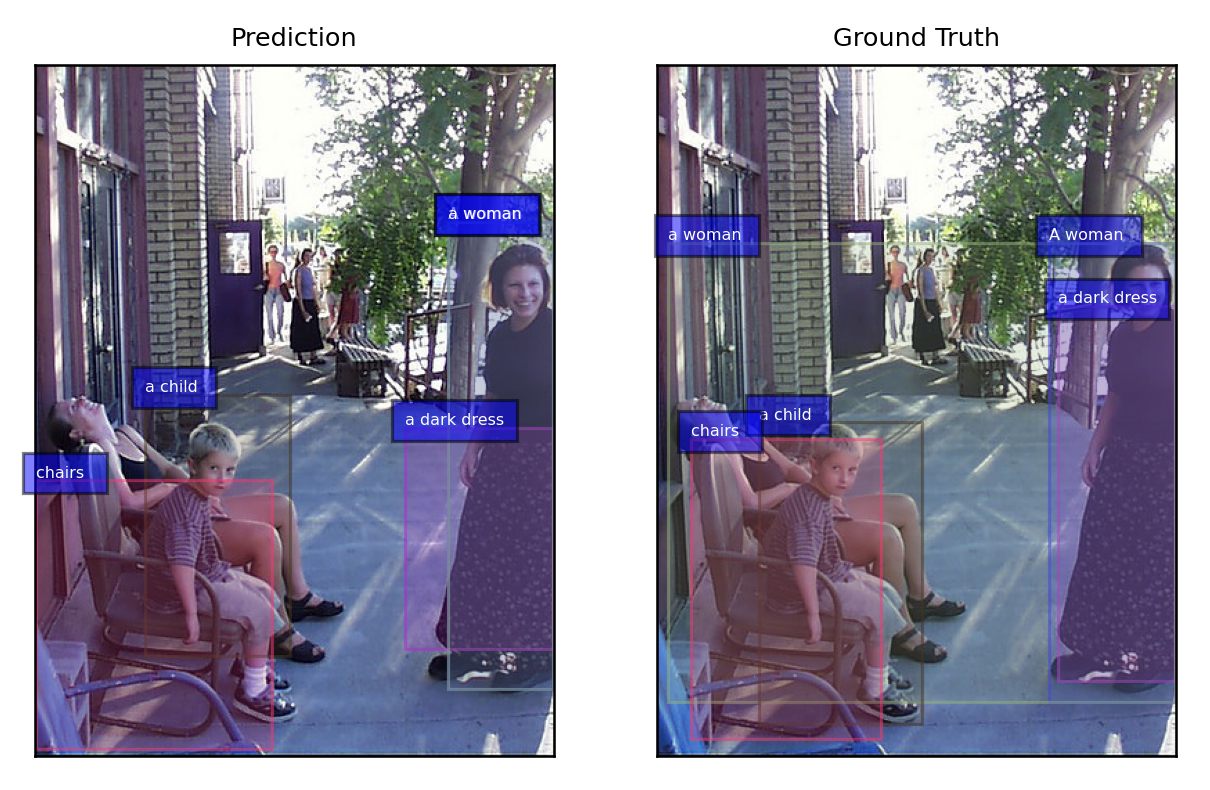
\includegraphics[width=0.8\textwidth]{figures/similing-woman.png}
  \caption[Model predictions for the image 102851549 from Flickr30k
    Entities]{ Model predictions for the image 102851549 given the
    sentence ``A woman in a dark dress smiles while a woman across
    from her and a child sit in chairs'' from Flickr30k Entities.
    Right side reports the ground truth bounding box while left side
    shows predictions.}
  \label{fig:qualitative-results}
\end{figure}

\subsection{Ablation Study}

To prove the effectiveness of concept similarity we trained the model
without applying concept similarity as prior. The
Tab.~\ref{tab:ablation-study} reports results. As we can see, concept
similarity is extremely helpful on both datasets and gives good
insight on what box to ground. By removing the prior on Flickr30k
Entities test set we got a worsening of $9\%$ absolute accuracy, while
on ReferIt this effect is even more noticeable: the worsening is of
$18.5\%$ absolute accuracy. Indeed, ReferIt contains complex sentences
from a syntactic point of view: being able to extract information such
as the concept of the phrase may help the model localizing the related
proposal.

\begin{table}
  \centering
  \begin{tabular}{l|ccc}
    \toprule
    Prior & Dataset & Acc. (\%) & P. Acc (\%) \\
    \midrule
    no & Flickr30k Entities & $41.2$ & $68.1$ \\
    mean & Flickr30k Entities & $50.2$ & $82.3$ \\
    \midrule
    no & ReferIt & $18.5$ & $37.1$ \\
    mean & ReferIt & $37.0$ & $60.0$ \\
    \bottomrule
  \end{tabular}
  \caption[Ablation study on prior application for both Flickr30k
    Entities and ReferIt]{ Ablation study on prior application for
    both Flickr30k Entities and ReferIt.}
  \label{tab:ablation-study}
\end{table}
